The United States contributed more than $12.5\%$ to the total carbon emissions
in 2020 \cite{european_commission_joint_research_centre_ghg_2021}. In response
to growing climate concerns local, state, and national governmental bodies have
announced myriad supports for clean energy projects; however, when you add
lenses of environmental justice and life cycle analysis, these transitions might
result in displacement instead. In 2012 Richard York from the Oregon State
Department of Sociology and Environmental Studies published a study of the
50-year history of alternative-energy installations to our modern grid
asserting that "to displace 1 kWh of fossil-fuel electricity requires
generating more than 11 kWh of non-fossil-fuel electricity,"
\cite{york_alternative_2012}. This conversion was based on 6 models of fossil
fuel use from 1960-2009, accounting for levels of urbanization, manufacturing,
age, and a variety of energy technologies.

This result challenges the assumption that there is a one-to-one relationship
between energy facilities with comparable power. In 2019 York and co-author
Shannon Bell further developed this idea saying that such proportional
representation studies "do not focus their discussions on or graphically
present the absolute quantity of energy in their assessments of purported
energy transitions," \cite{york_energy_2019}. They demonstrate with Figure
\ref{fig:percent_total_energy} that the proportional representation misses that
the total demand for energy has dramatically increased since the Industrial
Revolution. What may have looked like a transition in the mid-1800s from
biofuels to coal is merely a displacement, and they show that the energy
consumption of biofuels has increased since the early 1900s.

\begin{figure}[!ht]
  \subfloat[Proportional Energy Use\label{fig:percent}]{%
    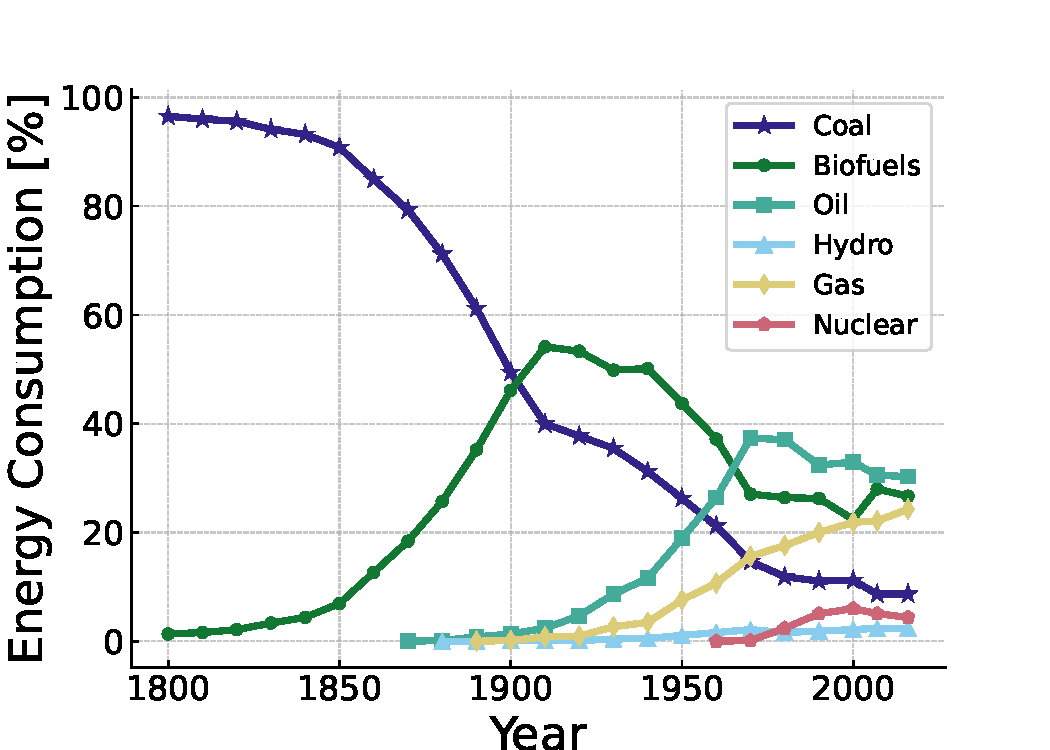
\includegraphics[width=0.495\textwidth]{images/leg_frame/proportional_fuel_use.pdf}
 }
  \hfill
  \subfloat[Total Energy Use\label{fig:total}]{%
    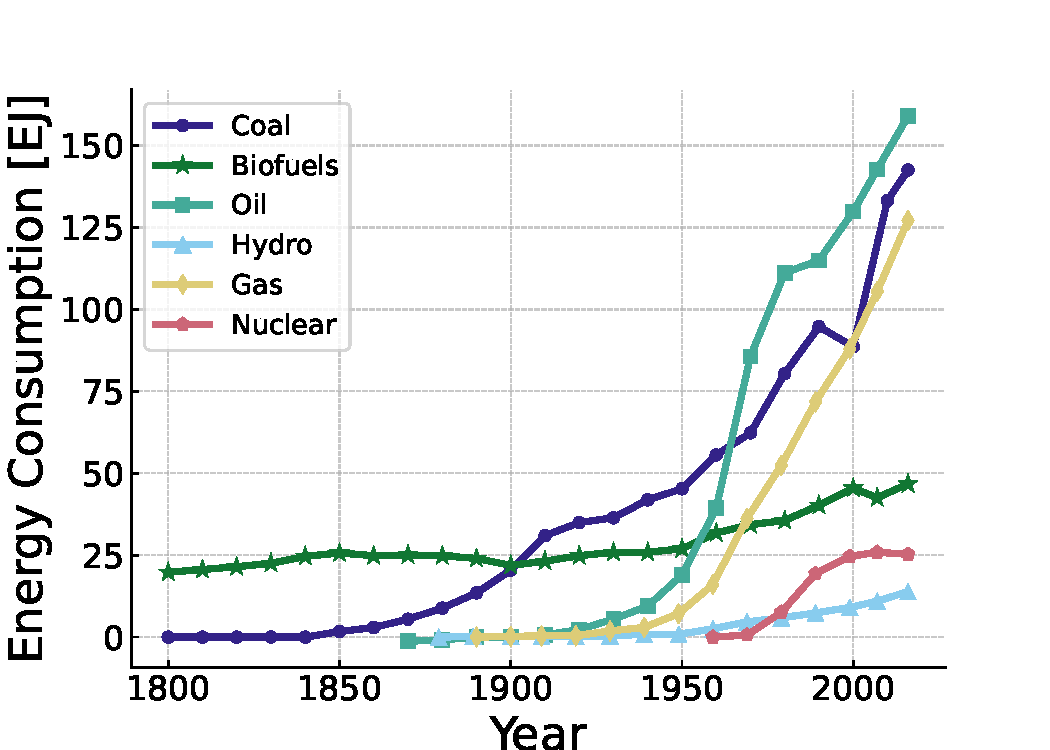
\includegraphics[width=0.495\textwidth]{images/leg_frame/total_fuel_use.pdf}
 }
  \caption{
    Global energy consumption (exajoules) by source. 1800--2017
    \cite{york_energy_2019}}
  \label{fig:percent_total_energy}
\end{figure}

Similarly, what looks in Figure \ref{fig:percent} like a transition away from
coal in the early 1900s, with the introduction of alternatives like oil and
hydroelectricity, belies the continued increase in coal consumption into the
early 2000s. If what we have axiomatically understood as a transition is not
happening, we arrive at the kernel of several grand challenges to our society
and our elected officials.

The policy inertia behind the monetary valuation of our energy system is
something that future generations could overcome, upending the incentives
policymakers might implement to drive an actual transition instead of a
displacement as we have discussed. If decision-makers focus on what a policy
will do only for the term of their service, they drastically undervalue the
impact that daily climate actions will have hundreds of years down the line. We
see this dichotomy in the 2020 grid failings in Texas during the unseasonably
cold front they experienced. From the outside, we can see how an extreme
weather event would create a great demand. This case is a microcosm of a
drastic change in the values a society had in an energy grid. In the span of a
couple of weeks a state that had proudly touted its achievement of a sustained
grid \cite{texas_ercot_nodate} experienced massive failures only for its
service to resume.

Since 2020, the \gls{ercot} has been working to update its grid to be more
resilient to such events, the Grid Deployment Office of \gls{doe} published a
report in 2024 outlining the more than \$270 billion of savings from increasing
connections to the Texas Interconnection
\cite{doe_transmission_planning_study_2024}. Concurrent with this announcement,
the \gls{doe} announced \$1.5 billion transmission investment that would go to
four projects in Texas, New Mexico, Louisiana, Mississippi, Maine, Oklahoma,
and Arizona \cite{doe_tran_announce_2024}. These projects are expected to be
completed by 2026 and will increase the capacity of the grid by 1.5 GW. This is
a step in the right direction, but it is not enough to ensure that the grid
will be resilient to future extreme weather events.

We can legislate for such changes by developing policy frameworks that bring in
the community and ask for continuous feedback. Elisa Papadis and George
Tsatsaronis set out to update the vision for a well-designed policy package in
their 2020 paper, surmising that producing policy "with measures such as
carefully introduced targeted investment subsidies, performance standards and
mandates, communication and education campaigns and a CO$_2$ tax for global
aviation and shipping" constitutes achieving this legislative framework
\cite{papadis_challenges_2020}. This approach will require geographically
bespoke solutions that draw in stakeholders, and keep them in a perpetual
feedback cycle where their changing values are reflected in updates. They go on
to advocate for expansion and investment in the massively complex \gls{usa}
power grid due to the requirements of more flexibly generated capacity.

Flexibility is a seemingly ubiquitous goal of decarbonized industries, like
chemical producers, which highlight big emitters that are large volume/
low-profit goods (disincentivizing development)
\cite{mallapragada_decarbonization_2023} or farm researchers who highlight the
growing importance of human intervention as climate change impacts their crop
in a negative feedback cycle \cite{farokhi_soofi_farm_2022}. The start is
focusing our efforts where investment can have the largest impact in the
shortest time, and to consult the changing valuation of stakeholders in how we
deploy electrification and updates to the grid.